% GNUPLOT: LaTeX picture with Postscript
\begingroup
  \makeatletter
  \providecommand\color[2][]{%
    \GenericError{(gnuplot) \space\space\space\@spaces}{%
      Package color not loaded in conjunction with
      terminal option `colourtext'%
    }{See the gnuplot documentation for explanation.%
    }{Either use 'blacktext' in gnuplot or load the package
      color.sty in LaTeX.}%
    \renewcommand\color[2][]{}%
  }%
  \providecommand\includegraphics[2][]{%
    \GenericError{(gnuplot) \space\space\space\@spaces}{%
      Package graphicx or graphics not loaded%
    }{See the gnuplot documentation for explanation.%
    }{The gnuplot epslatex terminal needs graphicx.sty or graphics.sty.}%
    \renewcommand\includegraphics[2][]{}%
  }%
  \providecommand\rotatebox[2]{#2}%
  \@ifundefined{ifGPcolor}{%
    \newif\ifGPcolor
    \GPcolortrue
  }{}%
  \@ifundefined{ifGPblacktext}{%
    \newif\ifGPblacktext
    \GPblacktexttrue
  }{}%
  % define a \g@addto@macro without @ in the name:
  \let\gplgaddtomacro\g@addto@macro
  % define empty templates for all commands taking text:
  \gdef\gplbacktext{}%
  \gdef\gplfronttext{}%
  \makeatother
  \ifGPblacktext
    % no textcolor at all
    \def\colorrgb#1{}%
    \def\colorgray#1{}%
  \else
    % gray or color?
    \ifGPcolor
      \def\colorrgb#1{\color[rgb]{#1}}%
      \def\colorgray#1{\color[gray]{#1}}%
      \expandafter\def\csname LTw\endcsname{\color{white}}%
      \expandafter\def\csname LTb\endcsname{\color{black}}%
      \expandafter\def\csname LTa\endcsname{\color{black}}%
      \expandafter\def\csname LT0\endcsname{\color[rgb]{1,0,0}}%
      \expandafter\def\csname LT1\endcsname{\color[rgb]{0,1,0}}%
      \expandafter\def\csname LT2\endcsname{\color[rgb]{0,0,1}}%
      \expandafter\def\csname LT3\endcsname{\color[rgb]{1,0,1}}%
      \expandafter\def\csname LT4\endcsname{\color[rgb]{0,1,1}}%
      \expandafter\def\csname LT5\endcsname{\color[rgb]{1,1,0}}%
      \expandafter\def\csname LT6\endcsname{\color[rgb]{0,0,0}}%
      \expandafter\def\csname LT7\endcsname{\color[rgb]{1,0.3,0}}%
      \expandafter\def\csname LT8\endcsname{\color[rgb]{0.5,0.5,0.5}}%
    \else
      % gray
      \def\colorrgb#1{\color{black}}%
      \def\colorgray#1{\color[gray]{#1}}%
      \expandafter\def\csname LTw\endcsname{\color{white}}%
      \expandafter\def\csname LTb\endcsname{\color{black}}%
      \expandafter\def\csname LTa\endcsname{\color{black}}%
      \expandafter\def\csname LT0\endcsname{\color{black}}%
      \expandafter\def\csname LT1\endcsname{\color{black}}%
      \expandafter\def\csname LT2\endcsname{\color{black}}%
      \expandafter\def\csname LT3\endcsname{\color{black}}%
      \expandafter\def\csname LT4\endcsname{\color{black}}%
      \expandafter\def\csname LT5\endcsname{\color{black}}%
      \expandafter\def\csname LT6\endcsname{\color{black}}%
      \expandafter\def\csname LT7\endcsname{\color{black}}%
      \expandafter\def\csname LT8\endcsname{\color{black}}%
    \fi
  \fi
  \setlength{\unitlength}{0.0500bp}%
  \begin{picture}(7200.00,5040.00)%
    \gplgaddtomacro\gplbacktext{%
      \csname LTb\endcsname%
      \put(588,2675){\makebox(0,0)[r]{\strut{}0.4}}%
      \put(588,2985){\makebox(0,0)[r]{\strut{}0.6}}%
      \put(588,3295){\makebox(0,0)[r]{\strut{}0.8}}%
      \put(588,3605){\makebox(0,0)[r]{\strut{}1.0}}%
      \put(588,3915){\makebox(0,0)[r]{\strut{}1.2}}%
      \put(588,4225){\makebox(0,0)[r]{\strut{}1.4}}%
      \put(588,4535){\makebox(0,0)[r]{\strut{}1.6}}%
      \put(720,2300){\makebox(0,0){\strut{}}}%
      \put(1872,2300){\makebox(0,0){\strut{}}}%
      \put(3024,2300){\makebox(0,0){\strut{}}}%
      \put(4175,2300){\makebox(0,0){\strut{}}}%
      \put(5327,2300){\makebox(0,0){\strut{}}}%
      \put(6479,2300){\makebox(0,0){\strut{}}}%
      \put(-50,3527){\rotatebox{-270}{\makebox(0,0){\strut{}$M^b_{\rm NS}$ ($M_{\odot}$)}}}%
    }%
    \gplgaddtomacro\gplfronttext{%
      \csname LTb\endcsname%
      \put(5492,4362){\makebox(0,0)[r]{\strut{}Hempel DD2 M=1.2}}%
      \csname LTb\endcsname%
      \put(5492,4142){\makebox(0,0)[r]{\strut{}Hempel DD2 M=1.4}}%
      \csname LTb\endcsname%
      \put(5492,3922){\makebox(0,0)[r]{\strut{}G. Shen FSU 2.1, M=1.2}}%
      \csname LTb\endcsname%
      \put(5492,3702){\makebox(0,0)[r]{\strut{}G. Shen FSU 2.1, M=1.4}}%
      \csname LTb\endcsname%
      \put(5492,3482){\makebox(0,0)[r]{\strut{}SFHo M=1.2}}%
    }%
    \gplgaddtomacro\gplbacktext{%
      \csname LTb\endcsname%
      \put(588,727){\makebox(0,0)[r]{\strut{}1}}%
      \put(588,951){\makebox(0,0)[r]{\strut{}2}}%
      \put(588,1175){\makebox(0,0)[r]{\strut{}3}}%
      \put(588,1399){\makebox(0,0)[r]{\strut{}4}}%
      \put(588,1623){\makebox(0,0)[r]{\strut{}5}}%
      \put(588,1847){\makebox(0,0)[r]{\strut{}6}}%
      \put(588,2071){\makebox(0,0)[r]{\strut{}7}}%
      \put(588,2295){\makebox(0,0)[r]{\strut{}8}}%
      \put(720,283){\makebox(0,0){\strut{}-4}}%
      \put(1872,283){\makebox(0,0){\strut{}-2}}%
      \put(3024,283){\makebox(0,0){\strut{} 0}}%
      \put(4175,283){\makebox(0,0){\strut{} 2}}%
      \put(5327,283){\makebox(0,0){\strut{} 4}}%
      \put(6479,283){\makebox(0,0){\strut{} 6}}%
      \put(6611,958){\makebox(0,0)[l]{\strut{}1e-02}}%
      \put(6611,1412){\makebox(0,0)[l]{\strut{}2e-02}}%
      \put(6611,1867){\makebox(0,0)[l]{\strut{}3e-02}}%
      \put(6611,2322){\makebox(0,0)[l]{\strut{}4e-02}}%
      \put(214,1511){\rotatebox{-270}{\makebox(0,0){\strut{}$dt/dT$ ($M_{\odot} \cdot {\rm hr}^{-1}$)}}}%
      \put(7512,1511){\rotatebox{-270}{\makebox(0,0){\strut{}$dt/dT$ (${\rm ms} \cdot {\rm hr}^{-1}$)}}}%
      \put(3599,-47){\makebox(0,0){\strut{}$t - t_{\rm merge}$ (ms)}}%
    }%
    \gplgaddtomacro\gplfronttext{%
    }%
    \gplgaddtomacro\gplbacktext{%
      \csname LTb\endcsname%
      \put(2748,1512){\makebox(0,0)[r]{\strut{} 0.25}}%
      \put(2748,1764){\makebox(0,0)[r]{\strut{} 0.5}}%
      \put(2748,2015){\makebox(0,0)[r]{\strut{} 0.75}}%
      \put(2880,1040){\makebox(0,0){\strut{}-0.25}}%
      \put(3600,1040){\makebox(0,0){\strut{} 0.25}}%
      \put(4319,1040){\makebox(0,0){\strut{} 0.75}}%
      \put(4451,1464){\makebox(0,0)[l]{\strut{}1e-03}}%
      \put(4451,1669){\makebox(0,0)[l]{\strut{}2e-03}}%
      \put(4451,1873){\makebox(0,0)[l]{\strut{}3e-03}}%
      \put(4451,2078){\makebox(0,0)[l]{\strut{}4e-03}}%
    }%
    \gplgaddtomacro\gplfronttext{%
    }%
    \gplbacktext
    \put(0,0){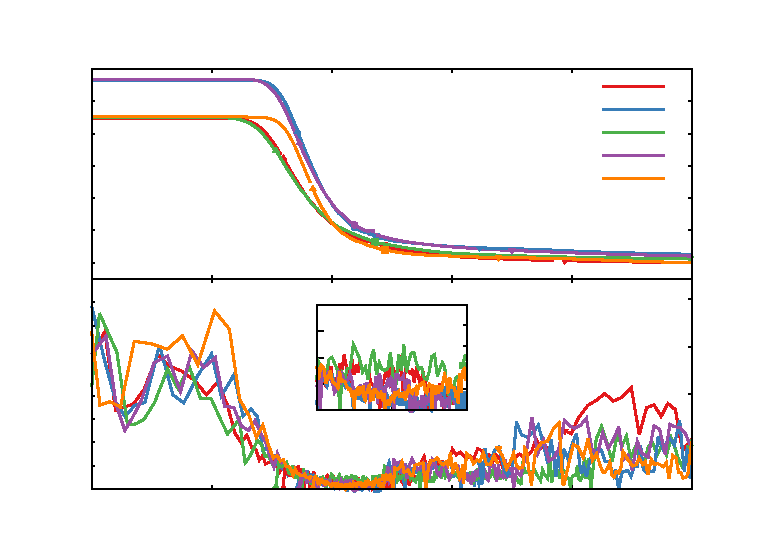
\includegraphics{images/mp-restmass-and-performance}}%
    \gplfronttext
  \end{picture}%
\endgroup
